\documentclass[11pt]{article}

\usepackage{amssymb}
\usepackage{amsmath}
\usepackage{graphicx}
\usepackage{cite}
\usepackage{xparse}
\usepackage[table]{xcolor}
%\usepackage{algorithmic}
%\usepackage{algorithm}
\usepackage{todonotes}
\usepackage{url}
\usetikzlibrary{arrows}
\usepackage{booktabs}
\usepackage{tikz}
\usetikzlibrary{calc,fit,shapes}

\usepackage{caption}
\usepackage{subcaption}


\usepackage{listings}
 \lstset{
            language=Matlab,                                % choose the language of the code
    %       basicstyle=10pt,                                % the size of the fonts that are used for the code
            numbers=left,                                   % where to put the line-numbers
            numberstyle=\footnotesize,                      % the size of the fonts that are used for the line-numbers
            stepnumber=1,                                           % the step between two line-numbers. If it's 1 each line will be numbered
            numbersep=5pt,                                  % how far the line-numbers are from the code
    %       backgroundcolor=\color{white},          % choose the background color. You must add \usepackage{color}
            showspaces=false,                               % show spaces adding particular underscores
            showstringspaces=false,                         % underline spaces within strings
            showtabs=false,                                         % show tabs within strings adding particular underscores
    %       frame=single,                                           % adds a frame around the code
    %       tabsize=2,                                              % sets default tabsize to 2 spaces
    %       captionpos=b,                                           % sets the caption-position to bottom
            breaklines=true,                                        % sets automatic line breaking
            breakatwhitespace=false,                        % sets if automatic breaks should only happen at whitespace
            escapeinside={\%*}{*)}                          % if you want to add a comment within your code
}


\setlength{\paperwidth}{8.5in}
\setlength{\paperheight}{11in}
\setlength{\voffset}{-0.2in}
\setlength{\topmargin}{0in}
\setlength{\headheight}{0in}
\setlength{\headsep}{0in}
\setlength{\footskip}{30pt}
\setlength{\textheight}{9.25in}
\setlength{\hoffset}{0in}
\setlength{\oddsidemargin}{0in}
\setlength{\textwidth}{6.5in}
\setlength{\parindent}{0in}
\setlength{\parskip}{9pt}

\newcommand{\ben}{\begin{enumerate}}
\newcommand{\een}{\end{enumerate}}

\DeclareGraphicsRule{.JPG}{eps}{*}{`jpeg2ps #1}

\title{Project: Streaming Graph Partitioning}
\author{Casey Battaglino\\Robert Pienta}
%\date{}
\begin{document}
\maketitle

\begin{abstract}
Graph partitioning is the process of dividing a graph into subgraphs such that the number of edges between subgraphs is reduced. Our project investigates the process of partitioning a graph using a \emph{streaming} partitioner, which must make partition decisions as each vertex is read from memory, simulating an online algorithm that must process nodes as they arrive. In this project, we demonstrate and analyze streaming graph partitioning on a wide spectrum of real-world and synthetic graphs, as well as explore ways of improving partition quality. 
\end{abstract}

\section{Graph Partitioning} \vspace{-10 pt}
Graph partitioning has been a standard problem in theoretical computer science for decades, but has seen increasing attention since the 1990s as a method of partitioning problems to increase parallel locality. The balanced graph partitioning problem can be stated as such: we wish to partition the nodes of a graph into $k$ components with capacity $(1+\epsilon)\frac{N}{k}$, such that cost is minimized, where cost is generally the number of edges that cross partition boundaries. While satisfying either the capacity constraint or the partitioning objective on their own is trivial, requiring both balance and cost-minimization places this problem in NP-complete, because it becomes a minimum-bisection problem~\cite{Garey:1979:CIG:578533}.

\begin{figure}[h]
\centering
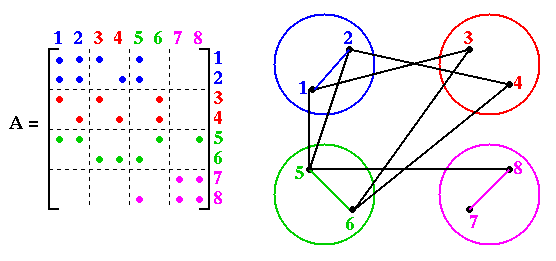
\includegraphics[scale=.60] {figures/graphpart.png}
\caption[Caption for]{Graph 4-partition shown with corresponding adjacency matrix \footnotemark}
\label{fig:0}
\end{figure}

\footnotetext{Source: Jim Demmel's CS267 Lectures,~\url{http://www.cs.berkeley.edu/~demmel/cs267}}

Offline graph partitioning algorithms, where the graph is allowed to exist in memory with total information about edges, have existed for decades. Hundreds of variants of such algorithms now exist, and range from spatial methods~\cite{Gilbert95geometricmesh} to spectral methods~\cite{arora2009expander}. The most scalable and effective graph partitioners on massive datasets are currently multi-level partitioners, which recursively contract the graph to a small number of vertices, and then heuristically optimize the problem on each subsequent expansion~\cite{karypis1998multilevel}. 

An effective partitioning can greatly increase the performance of sparse / graph algorithms. Consider a parallel Breadth-First Search where a graph's vertices (vertex edge lists) are partitioned between two machines. During each BFS step, each process must communicate all newly explored vertices to the owner of those vertices. Thus, for instance, in Figure~\ref{fig:0}, if we have 4 processes, all 14 nonzeros in the non-diagonal blocks must be communicated at some point. A good partitioner concentrates nonzeros in the diagonal blocks, thereby reducing communication (which is the main bottleneck in almost all graph computations). 

\section{Streaming Graph Partitioning}\vspace{-10 pt}
Streaming graph partitioning has only been introduced in the last couple of years~\cite{DBLP:journals/corr/abs-1212-1121,Stanton:2012:SGP:2339530.2339722,tsourakakis2012fennel}, as graphs grow to the point where they may not fit into memory, or must be distributed to compute nodes on the fly. In the streaming model, input data (vertices) arrive sequentially from a generating source (such as a web-crawler), and must be partitioned as they arrive.

Streaming partitioning is dependent on the order in which vertices arrive. For instance, a web crawler might generate vertices in an order that represents a Breadth-First or Depth-First traversal of the web, or we may receive vertices in a random order. An analysis of streaming algorithms may also consider an adversarial ordering that produces the worst possible results~\cite{Stanton:2012:SGP:2339530.2339722}. For the purposes of this project we always consider a random ordering, because in the literature it is always on par with or better than other orderings. 

\subsection{Streaming Heuristics}
Assuming vertices arrive in some order, a heuristic makes a partition decision, given vertex $v$, and capacity constraint $C$ (where $C$ is generally $\approx \frac{(\epsilon+|V|)}{n}$ Stanton presents the following heuristics, roughly in order from most naive to most complex~\cite{Stanton:2012:SGP:2339530.2339722}: (only the un-buffered heuristics are presented)

\begin{enumerate}
\item \textbf{Balanced:} assign $v$ to partition of minimum size, with random tie breaking.
\item \textbf{Chunking:} divide input stream into chunks of size $C$.
\item \textbf{Hashing:} assign $v$ to $H(v)$, where $H$ is hash function $F:V\to\{1\dots k\}$
\item \textbf{Weighted Deterministic Greedy (WDG):} Assign $v$ to partition that it has most edges to, weighted by the relative size of each partition (weight function can be linear or exponential).
\item \textbf{Weighted Randomized Greedy:} Assign $v$ randomly according to a probability distribution defined by the weights of each partition in WDG.
\item \textbf{Weighted Triangles:} Assign $v$ to partition whose intersection with $v$ contains the most triangles, weighted by the relative size of each partition.
\item \textbf{Balance Big:} for high-degree $v$, use Balanced. For low-degree $v$, use WDG. 
\end{enumerate}

Of note is that many major graph-processing toolkits such as GraphLab~\cite{Low:2012:DGF:2212351.2212354} use the hashed (random) partitioning method, which essentially produces a worst-case edgecut of size $\frac{k-1}{k}|E|$, but which has the benefit that $H(v)$ can be called at any time to return the compute node that owns $v$. 

In Stanton's experimental results~\cite{Stanton:2012:SGP:2339530.2339722}, WDG performed far better than any other partitioner. FENNEL~\cite{tsourakakis2012fennel} is a heuristic that generalizes the WDG partitioner for any weight function, and provides a somewhat more rigorous theoretical framework. For this project, we always consider a WDG partitioner. 

\subsection{Why Use Streaming Partitioning?}
The most salient property of streaming partitioning is its speed: it can partition the graph in a single sweep, with $O(|E|)$ memory access, storage, and run time. Existing graph partitioners require the whole graph to be represented in memory, whereas streaming graph partitioning can process vertices as they arrive.

As an example, partitioning a 26GB Twitter follower graph can take nearly a day using the fastest offline algorithms, but can take a matter of minutes using a streaming algorithm, with similar partition quality~\cite{tsourakakis2012fennel}. This also suggests that we could do multiple passes of a streaming partitioner (using the same or different heuristics) to further improve the partitioning, all in a fraction of the time that an offline partitioner would take to terminate. 

\section{Implementation}
Our first goal was to implement the generalized WDG partitioner FENNEL, and test it on a wide variety of real-world and synthetic graphs. Our initial `test-bed' was implemented in MATLAB, because many important properties of graphs can be easily extracted using vector notation on their adjacency matrices. As we scaled to larger graphs, the outer for-loop in the code (which iterates over each vertex) began to take an infeasible amount of time, so we implemented a more fully-featured test-bed in C. Our MATLAB and C code is located at~\url{https://github.com/cjbattagl/graphpart/}. The C code makes significant use of BeBoP's Sparse Matrix Converter:~\url{http://bebop.cs.berkeley.edu/smc/}.

\subsection{Features}
Our implementation can read graphs in three formats (Harwell-Boeing, Matlab, and Matrix-Market Formats). This allows us to read in the entire SNAP graph archive~\cite{Leskovec-data}. It can read in symmetric (undirected) and unsymmetric (directed) graphs. Once the graph is read in, we convert it from unordered triplet format to Compressed Sparse Row format, which allows us to iterate through the neighbor list of any node in linear time, as well as compute the degree of any node in constant time.

Once we have our graph stored as a matrix in CSR form, we can perform a simulation of streaming $k-$partitioning. First we generate the traversal order of the graph (a random vertex order, which we generate using a Knuth Shuffle). We maintain a data structure that contains the assignment of every assigned vertex to its partition. Thus, for a given vertex, we can compute the number of edges from that vertex to each partition by iterating over each edge incident to the vertex. We also maintain a running total of vertices in each partition. This process lets us compute the FENNEL algorithm in $O(|E|)=O(nnz(A))$ time. 

\subsection{Evaluation}

We measured the overall quality of partitions by the \textit{fraction of cut edges} $\lambda$.
\begin{align}\lambda = \frac{\text{Number of edges cut by partition}}{\text{Total number of edges}}\end{align}

In general, we can compare this to the expected quality of a random $k-$partition. To estimate this we just assume that each block has the same density of nonzeros, so we compute the fraction of nonzeros expected to be in non-diagonal blocks:
\begin{align}\lambda_r = \frac{k^2 - k}{k^2} = \frac{k-1}{k} \end{align}

Any partitioner that produces a partition with $\lambda < \lambda_r$ has thus improved the parallel locality of the graph ordering, so we present $\lambda_{r,k}$ along with our results.

\subsubsection{SNAP Data Set}
The SNAP data set is a set of real-world networks collected by Jure Leskovec and collaborators~\cite{Leskovec-data}. Many networks in the collection are power-law and scale-free representatives of social networks (such as collaboration networks, citation networks, email networks, and web graphs). We consider these to be ideal targets for streaming partitioning, because these domains are producing the vast majority of the `big-data' that is difficult to partition using traditional methods. 

We also speculate (but have no proof) that the `random' structure of scale-free networks better suits the random quality of streaming graph partitioning, whereas a spatially-oriented graph would be poorly suited (for instance, in a grid, a streaming partitioner would create many local pockets for one particular partition, whereas a spatial partitioner would recognize that the graph could be geometrically bisected). 

In Figure~\ref{table:big} we show the main properties of graphs in the SNAP database, as well as the performance of our streaming partitioner on them, for $k=2$ and $k=8$. 

\begin{figure}
\caption{Basic properties of graphs in SNAP data set~\cite{Leskovec-data}, and $\lambda$ for one pass. $\lambda_{r,2}=0.5,\lambda_{r,8}=0.87$}
\rowcolors{2}{blue!05}{blue!15}
\centering
{ \begin{tabular}{ *7l }    \toprule
\label{table:big}
\emph{Data Set} & $N$ & $nnz$ & \emph{sym} & \emph{power-law?} & $\lambda, k=2$ & $\lambda, k=8$ \\\midrule 
amazon0302 & 262111 & 1234877 & no & yes & 0.202&0.37\\ 
amazon0312 & 400727 & 3200440 & no & yes & 0.212&0.38\\ 
amazon0505 & 410236 & 3356824 & no & yes & 0.206&0.37\\ 
amazon0601 & 403394 & 3387388 & no & yes & 0.203&0.36\\ 
as-735 & 7716 & 26467 & yes & yes & 0.207&0.44\\ 
as-Skitter & 1696415 & 22190596 & yes & yes & 0.166&0.324\\ 
ca-AstroPh & 18772 & 396160 & yes & yes & 0.232&0.413\\ 
ca-CondMat & 23133 & 186936 & yes & yes & 0.214&0.398\\ 
ca-GrQc & 5242 & 28980 & yes & yes & 0.128&0.241\\ 
ca-HepPh & 12008 & 237010 & yes & yes & 0.082&0.192\\ 
ca-HepTh & 9877 & 51971 & yes & yes & 0.202&0.378\\ 
cit-HepPh & 34546 & 421578 & no & yes & 0.343&0.646\\ 
cit-HepTh & 27770 & 352807 & no & yes & 0.360&0.605\\ 
cit-Patents & 3774768 & 16518948 & no & yes & 0.402&0.726\\ 
email-Enron & 36692 & 367662 & yes & yes & 0.132&0.407\\ 
email-EuAll & 265214 & 420045 & no & yes & 0.280&0.538\\ 
Oregon-1 & 11492 & 46818 & yes & yes & 0.224&0.406\\ 
Oregon-2 & 11806 & 65460 & no & yes & 0.185&0.429\\ 
p2p-Gnutella04 & 10879 & 39994 & no & yes & 0.415&0.747\\ 
roadNet-CA & 1971281 & 5533214 & yes & no & 0.186&0.36\\ 
roadNet-PA & 1090920 & 3083796 & yes & no & 0.188&0.36\\ 
roadNet-TX & 1393383 & 3843320 & yes & no & 0.185&0.358\\ 
soc-Epinions1 & 75888 & 508837 & no & yes & 0.173&0.34\\ 
soc-LiveJournal1 & 4847571 & 68993773 & no & yes &0.234& 0.463\\ 
soc-sign-epinions & 131828 & 841372 & no & yes &0.173&0.34\\ 
soc-Slashdot0811 & 77360 & 905468 & no & yes &0.179&0.417\\ 
soc-Slashdot0902 & 82168 & 948464 & no & yes &0.236&0.382\\ 
web-BerkStan & 685230 & 7600595 & no & yes &0.187&0.301\\ 
web-Google & 916428 & 5105039 & no & yes &0.189&0.336\\ 
web-NotreDame & 325729 & 1497134 & no & yes &0.204&0.345\\ 
web-Stanford & 281903 & 2312497 & no & yes &0.154&0.34\\ 
wiki-Talk & 2394385 & 5021410 & no & yes &0.411&0.752\\ 
wiki-Vote  & 8297 & 103689 & no & yes &0.409&0.688\\ 
 \hline
\end{tabular}\par
}
\end{figure}

As a note, the ratio of change in $\lambda$ from $k=2$ to $k=8$ was for the vast majority of cases within 1.5 and 2.2. This shows a decent deal of scalability.

We also note Figure~\ref{fig:4}, which illustrates the result of the streaming algorithm on a more spacial network (roadNet-CA). The `local' nonzeros are those points in the 8 diagonal blocks, while the `remote' edges are those outside. While a good partitioner would concentrate the vast majority of elements along the diagonal (which is possible because the graph has very high diameter), the streaming partitioner fails to recognize this quality, and each partition has vertices distributed somewhat randomly through the network. Nonetheless, the partition is decent (only 18 percent of edges are cut). 

\begin{figure}[h!]
\centering
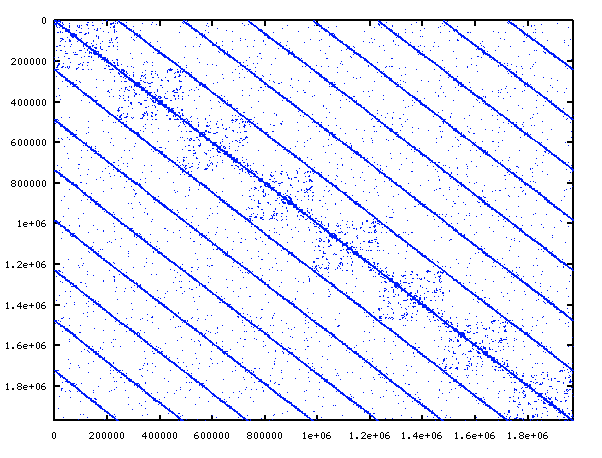
\includegraphics[scale=.60] {figures/roadNet-CA8.png}
\caption[Caption for]{Spy plot of roadNet-CA 8-partition ($\lambda=0.177$). This illustrates how a streaming algorithm cannot take into account the spatial/planar properties of a graph.}
\label{fig:4}
\end{figure}

\subsubsection{Synthetic Graphs}
To generate synthetic graphs we used the Stanford Network Analysis Platform (SNAP) random graph generator. 

\begin{figure}[h!]
\centering
  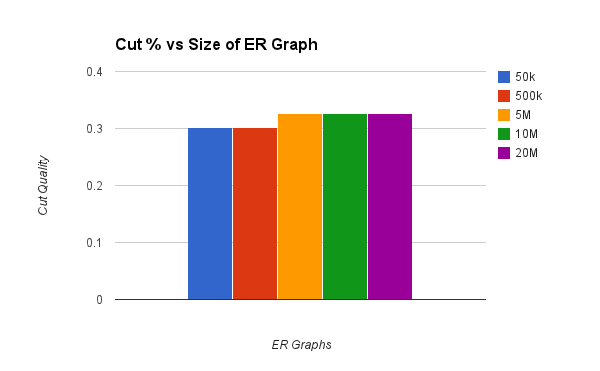
\includegraphics[width=.7\textwidth]{figures/lambda_ER.png}
  \caption{Partition quality of ER graphs with same $p$-value}
  \label{fig:lambdaer}
\end{figure}

\begin{figure}[h!]
\centering
  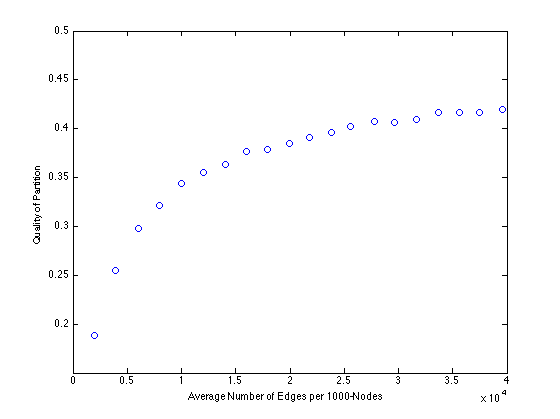
\includegraphics[width=.8\textwidth]{figures/varied_er_p.png}
  \caption{Partition quality of an ER graph with varying $p$-value, $k=2$}
  \label{fig:lambdap}
\end{figure}



In Figure~\ref{fig:lambdaer} we investigated the streaming graph partitioner on Erdos-Renyi graphs with a widely varying number of nodes, but the same probability $p$. From our small sample set, there appears to be little change in partition quality. 

In Figure~\ref{fig:lambdap} however, we increase the $p$-value on a single ER graph. We see that the partition quality significantly decreases. This is to be expected of all partitioners in general. In fact, for E-R graphs, the critical $p$-value for which the optimal edge cut is equal to the expected average random partition is relatively simple to identify~\cite{journals/cj/GanleyH94}

\section{Additional Passes}
Another operation we explored was performing additional passes of partitioning on a pre-partitioned graph. The reasoning is that the partitioner is fast enough that it may be faster to do $n$ passes than use a slower mainstream graph partitioner, for some value of $n$. To explore this idea, we perform a number of passes on the SNAP data set, and observe qualitatively which graphs benefit the most. 

The algorithm is simple: once we have computed the first partition, we retain the original partition mapping. Then, as we make another pass, we compute the new objective function using the partition mapping that has already been filled in. Vertices may then be switched to new partitions. This mitigates poor partitioning decisions that may have been made at the beginning of the algorithm, when there was not as much information. 

Figures~\ref{fig:01},\ref{fig:02},\ref{fig:03},\ref{fig:04} show the improvement of $\lambda$ as we continue to make passes over selected networks. Significant improvements are made for the vast majority of data sets.

We hope to contrast this performance to that of METIS in the future. (We have implemented a METIS partitioner for comparison but it currently encounters a segmentation faults with some frequency). 

%\begin{figure}[h]
%\centering
%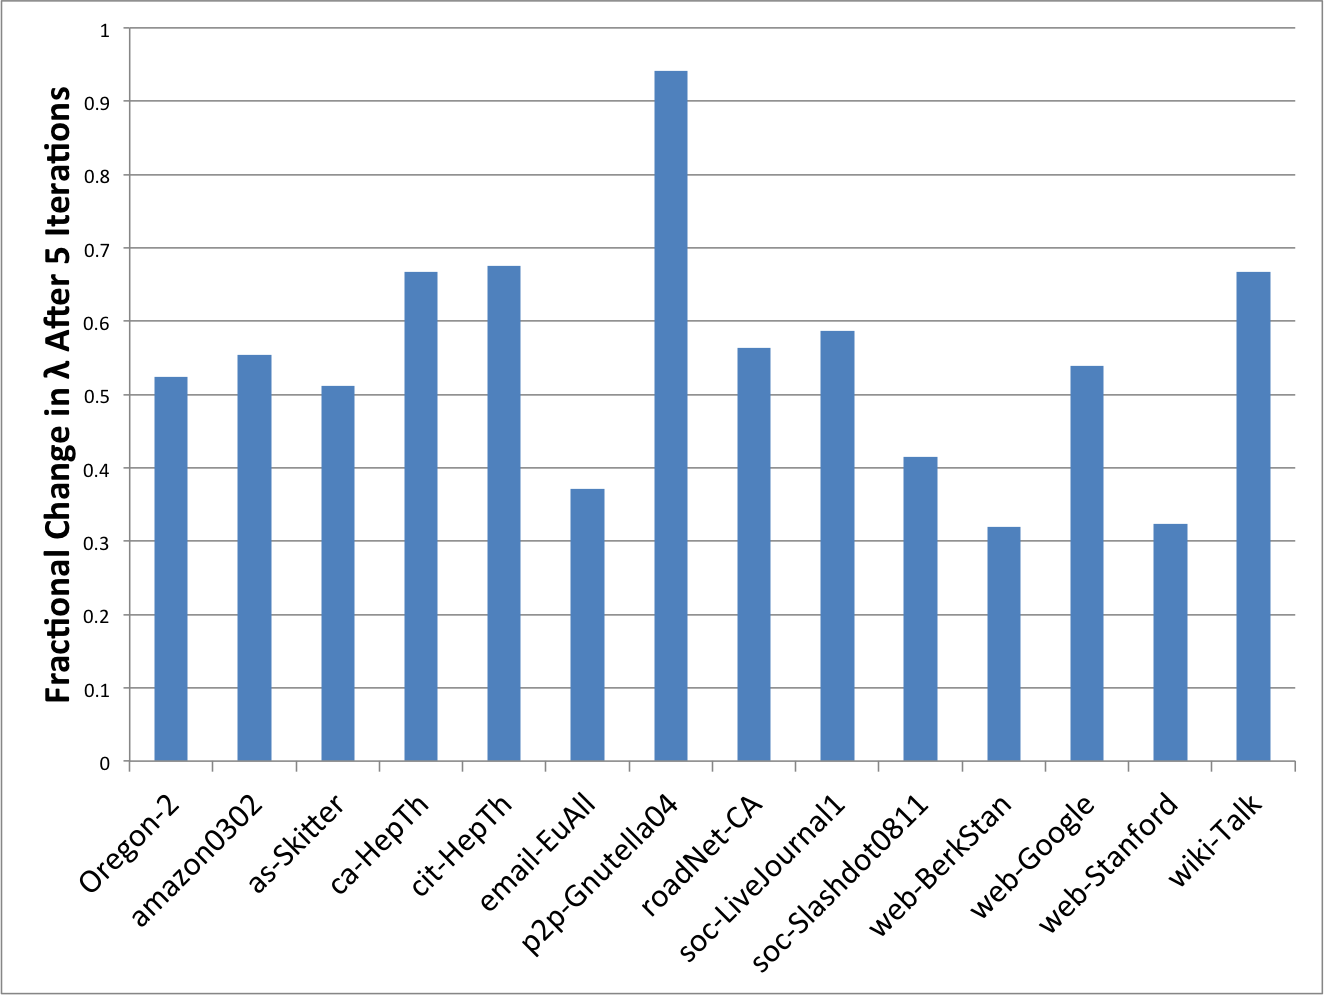
\includegraphics[scale=0.7] {figures/fracLambda.png}
%\caption[Caption for]{Improvement in $\lambda$ after 5 WDG passes.}
%\end{figure}

\begin{figure}[h!]
\centering
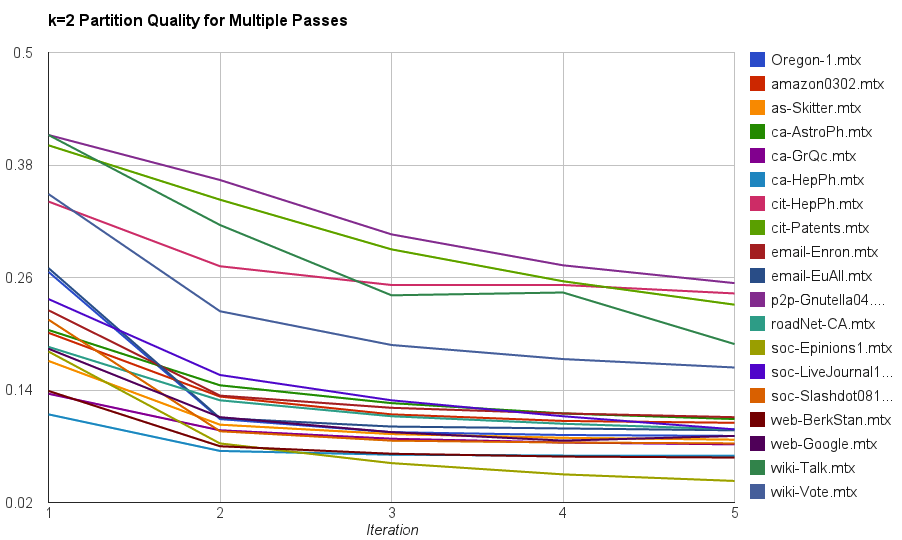
\includegraphics[scale=0.55] {figures/2partlambda}
\caption[Caption for]{Improvement in $\lambda$ over 5 WDG passes, $k=2$.}
\label{fig:01}
\end{figure}

\begin{figure}[h!]
\centering
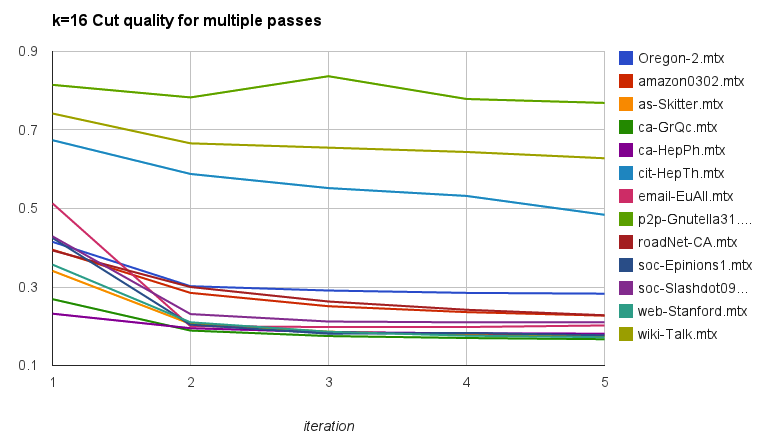
\includegraphics[scale=0.65] {figures/16partlambda}
\caption[Caption for]{Improvement in $\lambda$ over 5 WDG passes, $k=16$.}
\label{fig:02}
\end{figure}

\begin{figure}[h!]
\centering
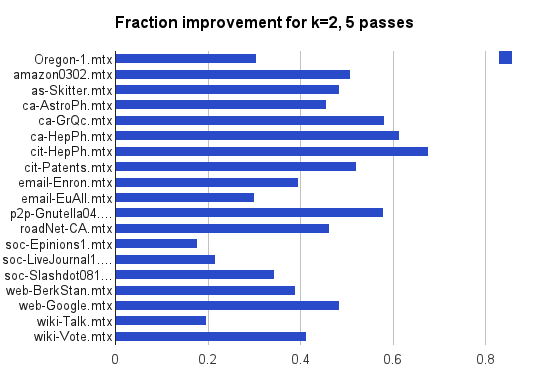
\includegraphics[scale=0.70] {figures/2partfrac}
\caption[Caption for]{Fraction Improvement in $\lambda$ after 5 WDG passes, $k=2$.}
\label{fig:03}
\end{figure}

\begin{figure}[h!]
\centering
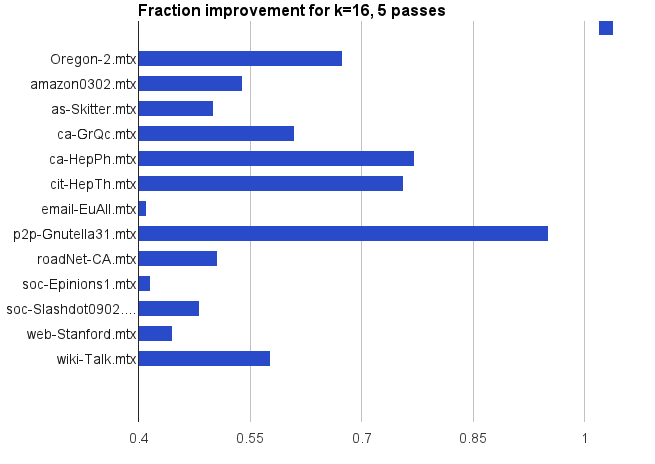
\includegraphics[scale=0.65] {figures/16partfrac}
\caption[Caption for]{Fraction Improvement in $\lambda$ after 5 WDG passes, $k=16$.}
\label{fig:04}
\end{figure}

\begin{figure}[h!]
\centering
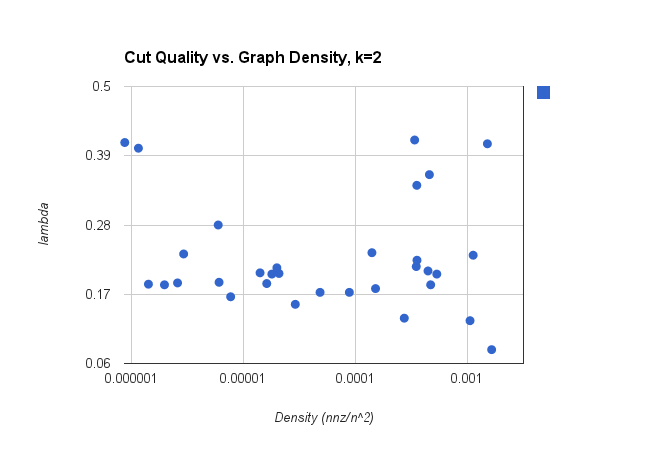
\includegraphics[scale=0.65] {figures/cutvsdens}
\caption[Caption for]{Cut quality vs nonzero density for each of the graphs in Figure~\ref{table:big}. The graph shows no noticeable correlation.}
\end{figure}

%\begin{figure}[h]
%\centering
%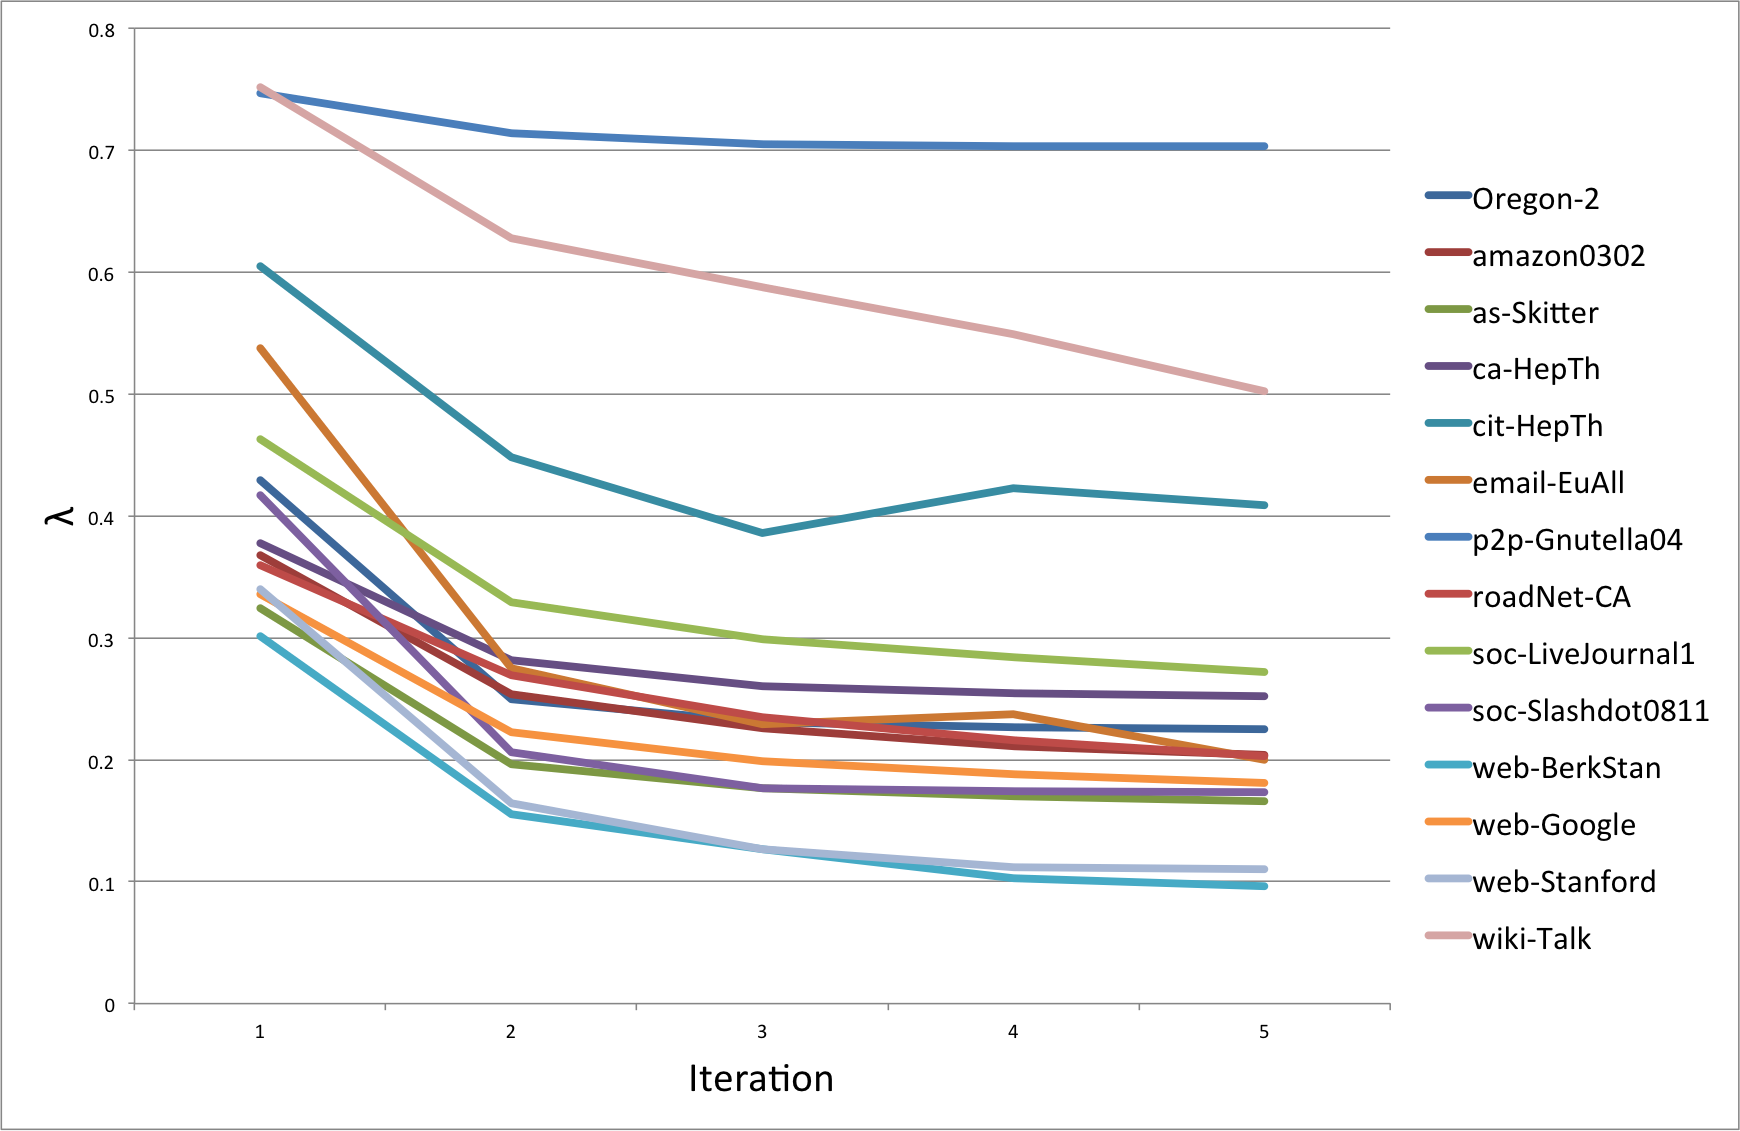
\includegraphics[scale=0.55] {figures/line_plot_lambda}
%\caption[Caption for]{$\lambda$ over multiple passes. $k=8, \lambda_r = 0.87$}
%\end{figure}

\section{Analysis}

One set of outlying (poorly-performing) data points we noticed was the Gnutella networks. While Gnutella networks exhibit power-law-like topology, elements of their algorithm truncate nodes from ever becoming extremely large. This does not match other social network topologies. The data sets also have extremely low clustering coefficient and a very small number of closed triangles. \cite{Ripeanu:2002:MGN:613352.613670}. This makes the Gnutella data set an anomaly compared to the others. 

Other data from real-world was harder to analyze -- there are not enough wide differences between data sets' results to draw strong conclusions. However, the encouraging side to this is that every partition was unexpectedly good. While Power-Law graphs are overwhelmingly considered to be difficult to partition~\cite{Abou-Rjeili:2006:MAP:1898953.1899055}, we have demonstrated that a very simple, fast, one-pass algorithm is capable of significantly reducing communication in their parallel computation, and that several further passes can further reduce edge cut by up to a factor of 3. Isolated comparisons we have made to the state-of-the-art partitioner METIS show that these results are competitive (usually within a factor of 2). This makes streaming partitioning a valid alternative to be integrated within distributed-memory, on-the-fly algorithms for big-data.

One interesting fact of note is that when we ran multiple passes on the graphs, one partition would become populated by very high-degree vertices. We see this in Figure~\ref{fig:dense}. We attribute this to the notion that scale-free graphs have a ``dense core'' surrounded by a less-dense periphery. This is qualitatively noticed when scale-free graphs are embedded in a spectral space~\cite{Lang04findinggood}. This dense partition tends to strongly emerge as we continue to make further passes of the streaming algorithm, and is what we attribute to the improvement in overall partition quality.

\begin{figure}[h!]
\centering
  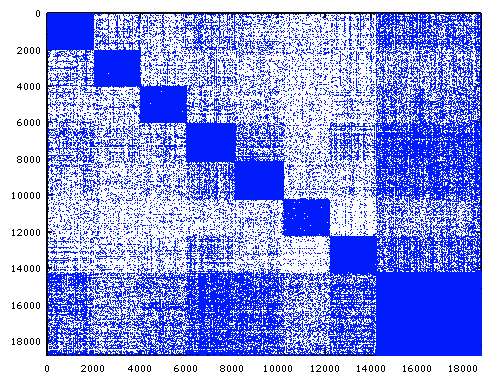
\includegraphics[width=.7\textwidth]{figures/astroPh8.png}
  \caption{Spy plot of ca-AstroPh 8-partition ($\lambda=0.253$). Note the denser, high-degree subgraph.}
  \label{fig:dense}
\end{figure}

\section{Future Work}
Our goal is adapt our C code into a distributed-memory streaming partitioner, and use it as a proof of concept that streaming partitioning is an effective way of increasing the performance of irregular, sparse distributed computations without taking a performance penalty. We are particularly interested in accelerating computations on large web- and social-network graphs. Along the way, we also wish to make a more critical comparison to METIS, in both partition quality and timing.


\newpage
\bibliographystyle{plain}
\bibliography{bib}

\appendix{Appendix A: C Code Example}
\subsection*{Partitioning kernel}
\begin{verbatim}
static int fennel_kernel(int n, int nparts, int *partsize, int *rowptr, int *colidx,
    bool **parts, float alpha, float gamma, int *emptyverts) {
      
  int *partscore = (int*)malloc(nparts * sizeof(int));
  int *row;
  int vert, k, s, nnz_row, best_part, randidx, nededges = 0, node = 0;
  float curr_score, best_score;
  int *vorder = genRandPerm(n);
  int oldpart;

  emptyverts = 0;

  for (int i = 0; i < n; i++) {
    for (s = 0; s < nparts; s++) { partscore[s]=0; }
    vert = vorder[i];
    row = &rowptr[vert];
    nnz_row = *(row+1) - *row;
    oldpart = -1;
   if(nnz_row != 0) {
      // generate partition scores for each partition
      for (k = *row; k < ((*row)+nnz_row); k++) {
        node = colidx[k];
        for (s = 0; s < nparts; s++) { if (parts[s][node] == 1) { partscore[s]++; }}
      }
        
      // choose optimal partition (initializing first)
      best_score = (partscore[0]-nnz_row) - calc_dc(alpha,gamma,partsize[0]);
      best_part = 0;
      for (s = 1; s < nparts; s++) {
        curr_score = (partscore[s]-nnz_row) - calc_dc(alpha,gamma,partsize[s]);
        if (curr_score > best_score) { best_score = curr_score; best_part = s; }
      }
      for (s = 0; s < nparts; s++) { 
        if (parts[s][vert] == 1) {
          oldpart = s;
        }
        parts[s][vert] = 0; 
      }
      parts[best_part][vert] = 1;
      partsize[best_part]++;
      if (oldpart >= 0) {
        partsize[oldpart]--;
      }
      
    } else { // empty vertex for some reason... assign it to random permutation
      emptyverts++;
      randidx = irand(nparts);
      for (s = 1; s < nparts; s++) {
        if (parts[s][vert] == 1) {
          oldpart = s;
        }
        parts[s][vert] = 0; 
      }
      parts[randidx][vert] = 1;
      partsize[randidx]++;
      if (oldpart >= 0) {
        partsize[oldpart]--;
      }
    }
  }
  
  free(vorder);
}
\end{verbatim}


\end{document}